\documentclass[11pt]{beamer}
\usetheme{CambridgeUS}
\usepackage[utf8]{inputenc}
\usepackage{amsmath}
\usepackage{amsfonts}
\usepackage{amssymb}
\usepackage{graphicx}
\usepackage{pgfpages}
\usepackage{framed}
\usepackage{xcolor}
\usepackage[most]{tcolorbox}
\usepackage{soul}
\usepackage{empheq}

% The replacement character � (often displayed as a black rhombus with a white
% question mark) is a symbol found in the Unicode standard at code point U
% +FFFD in the Specials table. It is used to indicate problems when a system 
% is unable to render a stream of data to a correct symbol.[4] It is usually 
% seen when the data is invalid and does not match any character. For this 
% reason we map explicitly this character to a blanck space.
\DeclareUnicodeCharacter{FFFD}{ }

\newcommand*{\itemimg}[1]{%
  \raisebox{-.3\baselineskip}{%
    \includegraphics[
      height=\baselineskip,
      width=\baselineskip,
      keepaspectratio,
    ]{#1}%
  }%
}

\newtcbox{\mymath}[1][]{%
    nobeforeafter, math upper, tcbox raise base,
    enhanced, colframe=blue!30!black,
    colback=blue!10, boxrule=1pt,
    #1}

\newcommand{\highlight}[1]{%
  \colorbox{yellow!50}{$\displaystyle#1$}}

\author{Giovanni Della Lunga\\{\footnotesize giovanni.dellalunga@unibo.it}}
\title{2.1 - Data Pre-Processing}
%\title{4.1 - Linear and Logistic Regression}
%\title{3.3 - Decision Trees}
%\title{6 - Text Vectorization}
%\title{7 - Classification for Text Analysis}
%\title{8 - Clustering for Text Similarity}
%\title{9 - Information Extraction}
\subtitle{} % (optional)
\setbeamercovered{transparent} 
\institute{Introduction to Machine Learning for Finance} 
\date{Bologna - February, 2022} 

\begin{document}

%\begin{frame}
%\includegraphics[width=\linewidth]{img/halloween-seminar-logo.PNG}
%\end{frame}

\begin{frame}
\titlepage
\end{frame}

\AtBeginSection[]
{
  %\begin{frame}<beamer>
  %\footnotesize	
  %\frametitle{Outline}
  %\begin{multicols}{2}
  %\tableofcontents[currentsection]
  %\end{multicols}	  
  %\normalsize
  %\end{frame}
  \begin{frame}
  \vfill
  \centering
  \begin{beamercolorbox}[sep=8pt,center,shadow=true,rounded=true]{title}  	\usebeamerfont{title}\insertsectionhead\par%
  \end{beamercolorbox}
  \vfill
  \end{frame}
}
\AtBeginSubsection{\frame{\subsectionpage}}
%
%---------------------------------------------------------------------------------------------------
%
\section{What is a decision tree}{}
%
%---------------------------------------------------------------------------------------------------
%
\begin{frame}{What is a Decision Tree}
	\begin{itemize}
		\item A \textbf{Decision Tree} shows a step-by-step process for making predictions;
		\item Example : if we are classifying bank loan application for a customer, the decision tree may look like this
Here we can see the logic how it is making the decision.
	\end{itemize}
	\begin{center}
	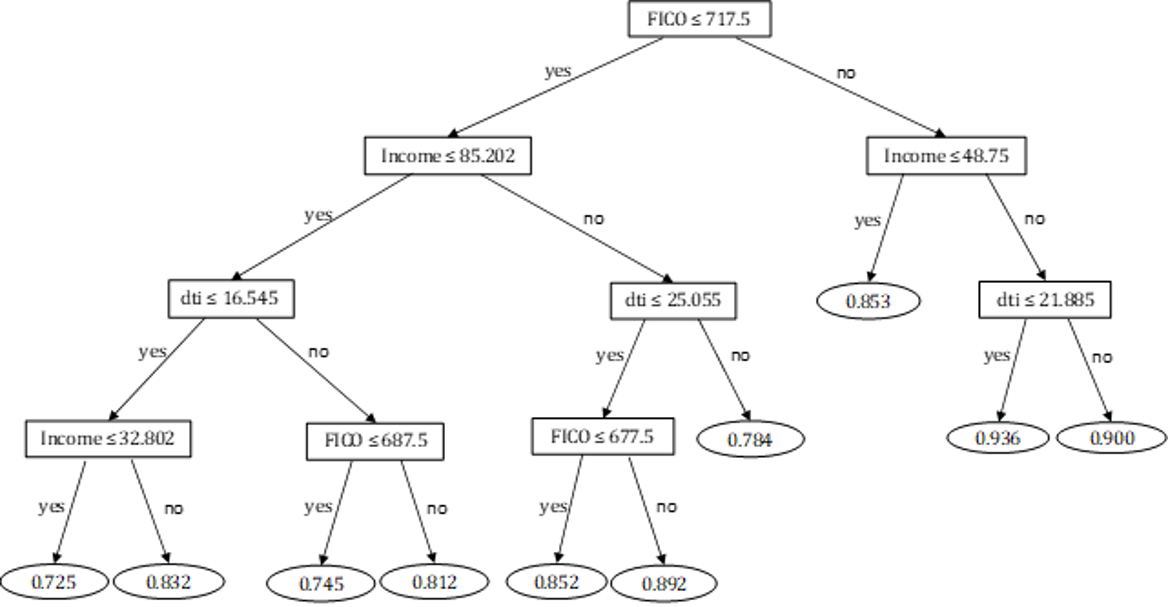
\includegraphics[scale=.3]{../05-pictures/lesson-3-3_pic_0.png}
	\end{center}
\end{frame}
%
%..................................................................
%
\begin{frame}{What is a Decision Tree}
	\begin{itemize}
		\item The decision is made by \textbf{considering features one at a time rather than all at once};
\item You will have different kind of splitting depending on the nature of the feature;
\item you can have a very simple decision tree in which the decision is a \textbf{boolean condition} (true, false) or you can have a \textbf{numeric data}
\item In the last case we have to define a desired \textbf{threshold} value of the feature. For instance, during each split of the parent node, we go to left node (with the corresponding subset of data) if a feature is less than the threshold, and right node otherwise.	
\end{itemize}
\end{frame}
%
%..................................................................
%
\begin{frame}{How to Build a Decision Tree}
	\begin{itemize}
	
 \item But how do we decide on the split? What is the best feature to select at the root node?
 \item and how we decide the threshold for numerical data?
		\item You can answer to both questions using the so called \textbf{information gain}
		\item But what is \textbf{information gain}?
	\end{itemize}
\end{frame}
%
%..................................................................
%
\begin{frame}{How to Build a Decision Tree}
\textbf{Impurity and Information Gain}
	\begin{itemize}
\item Decision trees use the concept of \textbf{impurity} to describe how homogeneous or “pure” a node is. 

\item A node is pure if all its samples belong to the same class, while a node with many samples from many different classes is called impure. 

\item The difference between the impurity of a node and that of the child nodes is called \textbf{Information Gain}. 
\end{itemize}

\vspace{.5cm}
The goal of a decision tree is, at each layer, to try to split the data into two (or more) groups, so that data that fall into the same group are most similar to each other (homogeneity), and groups are as different as possible from each other (heterogeneity).
\end{frame}
%
%..................................................................
%
\begin{frame}{How to Build a Decision Tree}
\begin{itemize}
\item In order to split the nodes at the most informative features, we need to define an
objective function that we want to optimize via the tree learning algorithm. 

\item Here,
our objective function is to maximize the \textbf{IG} at each split, which we define as follows:

\begin{equation}
IG(D_p, f) = I(D_p) - \sum\limits_{j=1}^m \frac{N_j}{N_p} I(D_j)
\end{equation}

Where: $f$ is the feature to perform the split, $D_p$ and $D_j$ are the dataset of the parent and $jth$ child node, $I$ is our impurity measure, 
$N_p$ is the total number of training examples at the parent node and $N_j$ is the number of examples in the jth child node. 

\end{itemize}
\end{frame}
%
%..................................................................
%
\begin{frame}{How to Build a Decision Tree}
\begin{itemize}
\item As we can see, the information gain is simply the difference between the impurity of the parent
node and the sum of the child node impurities—the lower the impurities of the child
nodes, the larger the information gain. 

\item However, for simplicity and to reduce the
combinatorial search space, most libraries (including scikit-learn) implement binary
decision trees. 

\item This means that each parent node is split into two child nodes, $D_{left}$
and $D_{right}$:

\begin{equation}
IG(D_p, f) = I(D_p) - \frac{N_{left}}{N_p}I(D_{left}) -
\frac{N_{right}}{N_p} I(D_{right})
\end{equation}
\end{itemize}
\end{frame}
%
%..................................................................
%
\begin{frame}{Measures of Information Gain}{How to Build a Decision Tree}
The three impurity measures or splitting criteria that are commonly used in binary decision trees are: 
\begin{itemize}
\item \textbf{Entropy}
\item \textbf{Gini Impurity}
\item \textbf{Classification Error} 
\end{itemize}
In the following we will focus only on the first two.
\end{frame}
%
%..................................................................
%
\begin{frame}{Shannon Entropy}
	\begin{itemize}
		\item Before taking on Shannon's definition of entropy, it might help to break down his definition of information. 
		\item The basic idea of Shannon's theory is that the informative value of a communicated message \textbf{depends on the degree to which the content of the message is surprising}. 
		\item Shannon considered a source generating some inputs $x$ characterised by a probability distribution $p(x)$. 
		
		\item Then he introduced the quantity

\begin{equation}
I_p(x) = log_2 \frac{1}{p(x)} = - log_2 \,p(x)
\end{equation}
\textbf{Information is uncertainty reduction} which in turn is just the inverse of the event?s probability.
	\end{itemize}
\end{frame}
%
%..................................................................
%
\begin{frame}{Shannon Entropy: Why the log?}
	\begin{itemize}
		\item Say, for example, that you have a simple binomial model completely random, with a 50/50 chance for a stock of being either up or down in the next interval $\Delta t$. 
		\item If someone tells you that the stock it?s going to be up tomorrow then they have actually reduced your uncertainty by a factor of two. \item There were two equally likely options, now there is just one.
		\item  In this case the "channel" (whatever it is) actually sent you a \textbf{single bit} of useful information:
		\begin{equation}
I_p(x) = - log_2 \, \frac{1}{2} = log_2 \, 2 = 1
\end{equation}

	\end{itemize}
\end{frame}
%
%..................................................................
%
\begin{frame}{Shannon Entropy: Why the log?}
	\begin{itemize}
		\item Now suppose the future asset price has actually 8 possible states, all equally likely. 
		\item Now when your insider gives you tomorrow?s price, he is dividing your uncertainty by a factor of 8, which is 2 to the power of 3. 
		\item So he sents you 3 bits of useful information. 
		\item Again, the number of bits of information that were actually communicated by computing the binary logarithm of the uncertainty reduction factor, which in this example is 8. 

	\end{itemize}
\end{frame}
%
%..................................................................
%
\begin{frame}{Shannon Entropy: Why the log?}
	\begin{itemize}
		\item But what if the possibilities are not equally likely? 
		\item Say 75\% chance up, and 25\% down. 
		\item If the insider tells you the asset it?s going to be down tomorrow, then your uncertainty has dropped by a factor of 4, which is 2 bits of information. 
\item Again the uncertainty reduction is just the inverse of the event?s probability, in this case the inverse of 25\% is 4 and the $log$ is 2. 
	\end{itemize}
\end{frame}
%
%..................................................................
%
\begin{frame}{Shannon Entropy: Why the log?}
	\begin{itemize}
		\item Now if the insider tells you the asset it?s going to be up tomorrow then your uncertainty hasn?t dropped much. 
		\item In fact, you get just about $0.41$ bits of information. 
		\item So how much information are you actually going to get from the insider, on average? 
		\item Well, there?s a 75\% chance that the asset will be up tomorrow, and you get in this case $0.41$ bits of information. 
		\item Then there?s a 25\% chance that it will be down, in which case  and this will give you 2 bits of information. 
		\item So on average, you will get $0.81$ bits of information from your insider. 

	\end{itemize}
\end{frame}
%
%..................................................................
%
\begin{frame}{Shannon Entropy}
	\begin{itemize}
		\item So what we just computed is called the \textbf{Entropy}. 
		\item It is a measure of how uncertain the events are.
	\end{itemize}

\begin{empheq}[box={\mymath[colback=red!20,drop lifted shadow, sharp corners]}]{equation*}
H(p) = - \sum\limits_{i=1}^n p_i \,\log(p_i)
\end{empheq}

\begin{tcolorbox}
Entropy measures the \textbf{average amount of information} that you get when you receive a signal from a transmission channel, or more generally the average amount of information that you get from one sample drawn from a given probability distribution $p$. It tells you how unpredictable that probability distribution is.
\end{tcolorbox}
\end{frame}
%
%..................................................................
%
\begin{frame}{Measures of Uncertainty}
	\begin{itemize}
		\item Suppose that there are $n$ possible outcomes and $p_i$ is the probability of outcome $i$ with $\sum\limits_{i=1}^n\, p_i=1$
		\item Entropy measure of uncertainty: $$\text{Entropy}=-\sum\limits_{i=1}^n\, p_i \,\ln(p_i)$$
		\item Gini Measure of uncertainty: $$\text{Gini} = 1 - \sum\limits_{i=1}^n p_i^2$$
	\end{itemize}
\end{frame}
%
%..................................................................
%
\begin{frame}{Information Gain}
	\begin{itemize}
		\item The information gain is the expected decrease in uncertainty (as measured by either entropy or Gini).
		\item Suppose that there is a 20\% chance that a person will receive a job offer 
		\item Suppose further that there is a 50\% chance the person has a relevant degree. If the person does have a relevant degree the probability of a job offer rises to 30\%, otherwise it falls to 10\%
	\end{itemize}
\end{frame}
%
%..................................................................
%
\begin{frame}{Information Gain}
$$\text{Initial Entropy} = -[0.2\,\log(0.2) + 0.8\,\log(0.8)]=0.7219$$
\vspace{0.5cm}
\begin{align*}\text{Expected Entropy} =&-0.5 \cdot [0.1 \log(0.1) + 0.9\log(0.9)]\\ &- 0.5 \cdot [0.3\log(0.3) + 0.7\log(0.7)] \\ &=0.6751\end{align*}    
The Expected information gain from knowing whether there is a relevant degree is $$ \text{gain}= 0.7219-0.6751=0.0468$$
\end{frame}
%
%..................................................................
%
\begin{frame}{The Decision Tree Algorithm}
	\begin{itemize}
		\item Algorithm \textbf{chooses the feature at the root of the tree that has the greatest expected information gain};
		\item At subsequent nodes it choose the feature (not already chosen) that has the greatest expected information gain;
		\item When there is a threshold, it determines the optimal threshold for each feature (i.e., the threshold that maximizes the expected information gain for that feature) and bases calculations on that threshold 
	\end{itemize}
\end{frame}
%
%---------------------------------------------------------------------------------------------------
%
\section{Application to credit decision}
%
%---------------------------------------------------------------------------------------------------
%
\begin{frame}{Introduction}
    \begin{itemize}
        \item The Lending Club case illustrates how decision trees can be applied to credit risk assessment.
        \item The goal is to predict whether a loan will default or not based on four key financial variables:
        \begin{itemize}
            \item Home Ownership (Categorical: 1 if owned, 0 if rented)
            \item Income (Numerical: annual income in dollars)
            \item Debt-to-Income Ratio (DTI) (Numerical: total monthly debt payments divided by gross monthly income)
            \item Credit Score (FICO Score) (Numerical: a measure of creditworthiness)
        \end{itemize}
        \item Training dataset: 8,695 observations (1,499 defaulted loans, 7,196 good loans)
    \end{itemize}
\end{frame}
%
%..................................................................
%
\begin{frame}{Step 1: Initial Entropy Calculation}
    \begin{itemize}
        \item Probability of a good loan:
        \[ P_{\text{good}} = \frac{7,196}{8,695} = 0.8276 \]
        \item Initial entropy:
        \[ H_{\text{initial}} = - (0.8276 \log 0.8276 + 0.1724 \log 0.1724) = 0.6632 \]
    \end{itemize}
	\begin{center}
	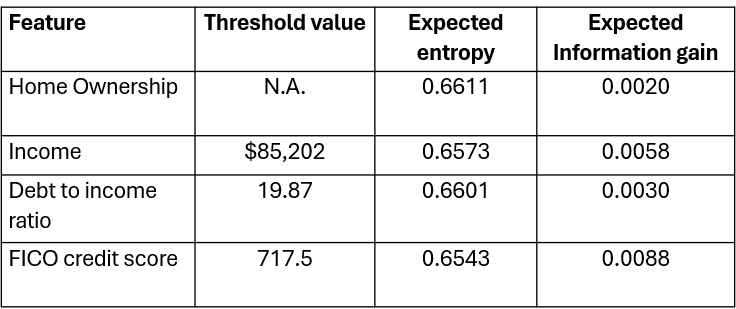
\includegraphics[scale=.5]{../05-pictures/lesson-3-3_pic_4.png}
	\end{center}
\end{frame}
%
%..................................................................
%
\begin{frame}{Step 2: Selecting the Root Node}
\footnotesize{
    \begin{table}[]
        \centering
        \begin{tabular}{|c|c|c|c|}
            \hline
            Feature & Threshold & Expected Entropy & Information Gain \\
            \hline
            Home Ownership & N.A. & 0.6611 & 0.0020 \\
            Income (\$000s) & 85.202 & 0.6573 & 0.0058 \\
            Debt-to-Income (\%) & 19.87 & 0.6601 & 0.0030 \\
            \textbf{Credit Score (FICO)} & \textbf{717.5} & \textbf{0.6543} & \textbf{0.0088} \\
            \hline
        \end{tabular}
    \end{table}
    }
    \begin{itemize}
        \item Since FICO Score at 717.5 has the highest information gain, it is selected as the root node.
    \end{itemize}
\end{frame}
%
%..................................................................
%
\begin{frame}{Step 3: Splitting the Tree}
	\begin{center}
	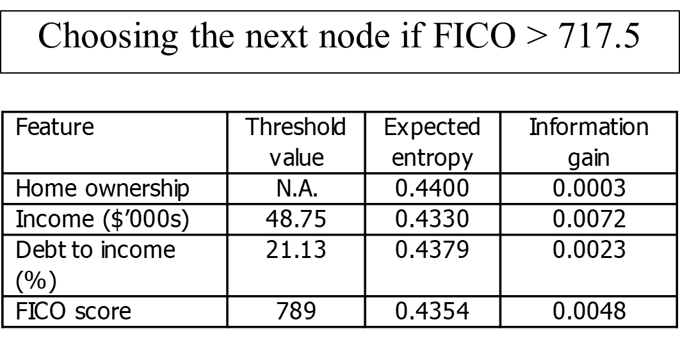
\includegraphics[scale=.5]{../05-pictures/lesson-3-3_pic_5.png}
	\end{center}
\end{frame}
%
%..................................................................
%
\begin{frame}{Step 3: Splitting the Tree}
	\begin{center}
	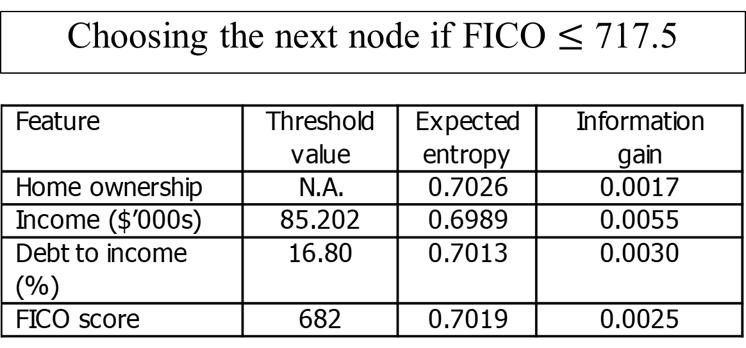
\includegraphics[scale=.5]{../05-pictures/lesson-3-3_pic_6.png}
	\end{center}
\end{frame}
%
%..................................................................
%
\begin{frame}{Step 3: Splitting the Tree}
    \begin{itemize}
        \item Further splits:
        \begin{itemize}
            \item If $FICO>717.5$ → Further split by $Income > 48.75K$
            \item If $FICO \le 717.5$ → Further split by $Income > 85.202K$ and $DTI \le 16.545\%$
        \end{itemize}
        \item Examples:
        \begin{itemize}
            \item If $FICO > 717.5$, $Income > 48.75K$, and $DTI > 21.885\%$, probability of no default = 0.900.
            \item If $FICO \le 717.5$, $Income \le 32.802K$, and $DTI \le 16.545\%$, probability of no default = 0.725.
        \end{itemize}
    \end{itemize}
\end{frame}
%
%..................................................................
%
\begin{frame}{Step 3: Splitting the Tree}
The construction of the tree continues in this way. The full tree produced
by Sklearn’s DecisionTreeClassifier is summarized in Figure.
	\begin{center}
	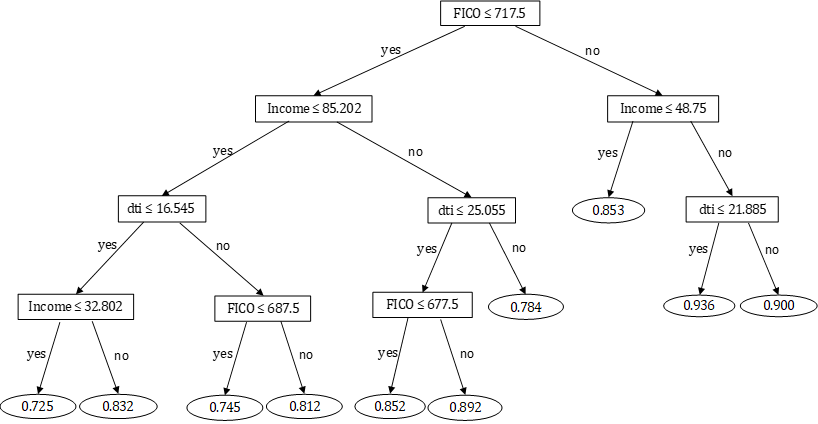
\includegraphics[scale=.5]{../05-pictures/lesson-3-3_pic_7.png}
	\end{center}
\end{frame}
%
%..................................................................
%
\begin{frame}{Step 3: Splitting the Tree}
The final points reached by the tree (shown as ovals) are referred to as
leaves. The numbers shown in the leaves in Figure are the predicted
probabilities of default.	
\begin{center}
	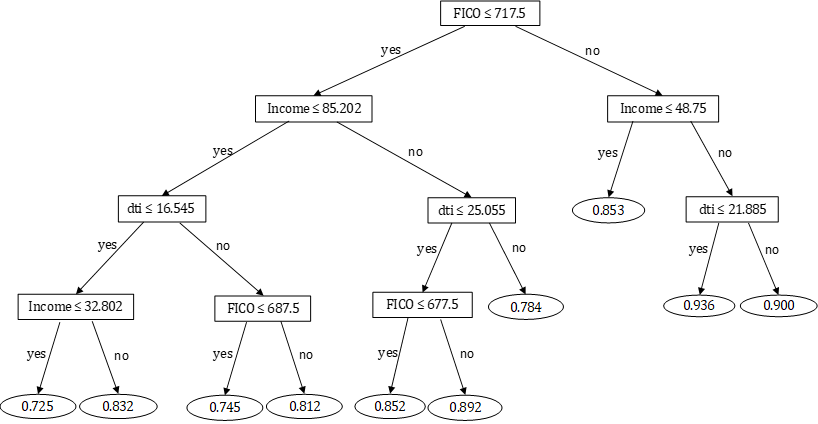
\includegraphics[scale=.5]{../05-pictures/lesson-3-3_pic_7.png}
	\end{center}
\end{frame}
%
%..................................................................
%
\begin{frame}{Step 3: Splitting the Tree}
\footnotesize{
 For example, if $FICO > 717.5$, $Income > 48.75$ and $dti > 21.885$, the estimated probability of no-default is 0.900. This is because there were 379 observations in the training set satisfying these
conditions and 341 of them were good loans (341/379 = 0.900)}	
\begin{center}
	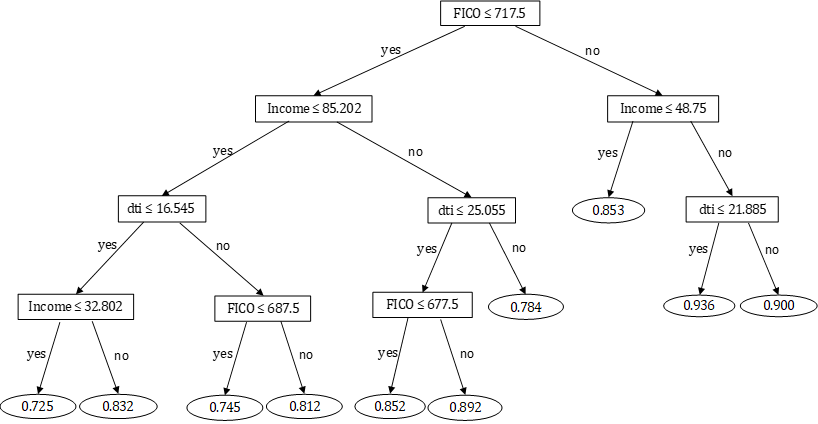
\includegraphics[scale=.5]{../05-pictures/lesson-3-3_pic_7.png}
	\end{center}
\end{frame}
%
%..................................................................
%
\begin{frame}{Step 4: Decision Thresholds and ROC Curve}
    \begin{itemize}
        \item A Z-value determines the threshold for classifying a loan as good.
        \item Three thresholds analyzed:
        \begin{itemize}
            \item \textbf{Z = 0.75}: Predicts that all loans are good except:
            \begin{itemize}
                \item $Income \le 85,202$, $DTI > 16.545$, $FICO \le 687.5$
                \item $Income \le 32,802$, $DTI \le 16.545$, $FICO \le 717.5$
            \end{itemize}
            \item \textbf{Z = 0.80}: Also excludes $FICO \le 717.5$, $Income > 85,202$, $DTI > 25.055$.
            \item \textbf{Z = 0.85}: Predicts loans as good only if:
            \begin{itemize}
                \item $FICO > 717.5$, or
                \item $FICO \le 717.5$, $Income > 85,202$, $DTI \le 25.055$.
            \end{itemize}
        \end{itemize}
    \end{itemize}
\end{frame}
%
%..................................................................
%
\begin{frame}{Step 5: Performance Evaluation}
    \begin{itemize}
        \item AUC (Area Under Curve) used to measure predictive performance:
        \begin{itemize}
            \item Decision Tree \textbf{AUC = 0.5948}
            \item Logistic Regression \textbf{AUC = 0.6020}
        \end{itemize}
        \item While logistic regression performs slightly better, decision trees offer interpretability.
    \end{itemize}
\begin{center}
	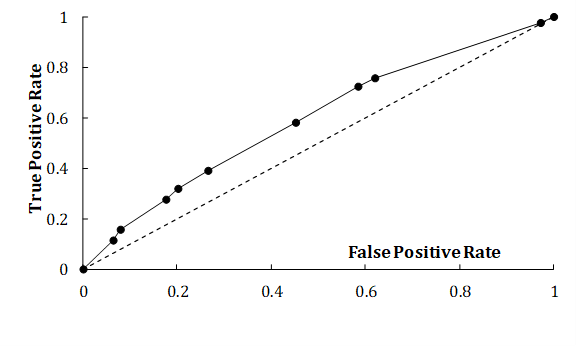
\includegraphics[scale=.5]{../05-pictures/lesson-3-3_pic_8.png}
	\end{center}
\end{frame}
%
%..................................................................
%
\begin{frame}{Conclusion}
    \begin{itemize}
        \item The decision tree approach to Lending Club loan classification demonstrates how financial variables influence creditworthiness.
        \item Highlights:
        \begin{itemize}
            \item The importance of the \textbf{FICO score} as the primary predictor.
            \item The trade-off between \textbf{precision and recall} when selecting a \textbf{Z-threshold}.
            \item The interpretability of decision trees compared to other models.
        \end{itemize}
        \item Provides a structured, data-driven method to assess lending risk.
    \end{itemize}
\end{frame}
%
%---------------------------------------------------------------------------------------------------
%
\section{Continuous Target Variables}
%
%---------------------------------------------------------------------------------------------------
%
\begin{frame}{Introduction}
    \begin{itemize}
        \item A \textbf{Decision Tree} can be used to predict continuous values using \textbf{Regression Trees}.
        \item Instead of making a \textbf{yes/no} decision like classification, a regression tree splits the data into smaller groups and assigns each group an \textbf{average value}.
    \end{itemize}
\end{frame}

\begin{frame}{Example: Predicting House Prices}
    \textbf{Dataset:}
    \begin{table}[]
    \begin{center}
        \begin{tabular}{|c|c|c|}
        \hline
        Size (m²) & Rooms & Price (\$) \\
        \hline
        50 & 2 & 100,000 \\
        60 & 2 & 120,000 \\
        70 & 3 & 150,000 \\
        90 & 3 & 200,000 \\
        100 & 4 & 220,000 \\
        \hline
        \end{tabular}
    \end{center}
	\end{table}
\end{frame}
%
%---------------------------------------------------------------------------------------------------
%
\begin{frame}{Finding the Best Split}
    \begin{itemize}
        \item We evaluate \textbf{every possible split} and choose the one that minimizes the \textbf{Mean Squared Error (MSE)}.
        \item Possible split points: 55, 65, 75, 85, 95, etc.
        \item The algorithm finds the split that results in the \textbf{lowest total error}.
    \end{itemize}
\end{frame}
%
%---------------------------------------------------------------------------------------------------
%
\begin{frame}{Mathematical Formulation}
    \textbf{Mean Squared Error (MSE):}
    \begin{equation}
        \text{MSE} = \frac{1}{n} \sum_{i=1}^{n} (y_i - \hat{y})^2
    \end{equation}
    where:
    \begin{itemize}
        \item $y_i$ is the actual value.
        \item $\hat{y}$ is the predicted value (average of the group).
        \item $n$ is the number of data points in the group.
    \end{itemize}
\end{frame}
%
%---------------------------------------------------------------------------------------------------
%
\begin{frame}{Example: Testing Split at 75m²}
    \begin{itemize}
        \item \textbf{Group 1 (Size $\leq$ 75m²)}
        \begin{itemize}
            \item Houses: 50, 60, 70
            \item Average Price: $123,333$
        \end{itemize}
        \item \textbf{Group 2 (Size $>$ 75m²)}
        \begin{itemize}
            \item Houses: 90, 100
            \item Average Price: $210,000$
        \end{itemize}
    \end{itemize}
\end{frame}
%
%---------------------------------------------------------------------------------------------------
%
\begin{frame}{Automating the Process with Python}

Decision tree algorithms like \textbf{CART (Classification and Regression Trees)} automatically find the best split. The optimal split point found was \textbf{80m²}. Below is a visualization of the Decision Tree Regression model.

    \begin{center}
        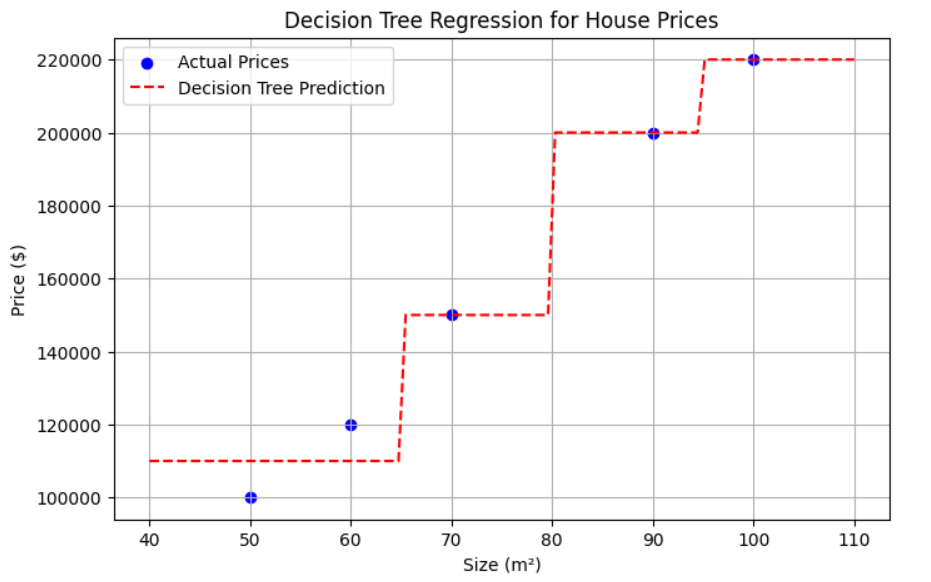
\includegraphics[width=0.8\linewidth]{../05-pictures/lesson-3-3_pic_9.png}
    \end{center}
\end{frame}
%
%---------------------------------------------------------------------------------------------------
%
\begin{frame}{Using the Tree for Prediction}
    \begin{itemize}
        \item To predict a new value, we follow the tree’s splits based on the input features.
        \item Example: If we want to predict the price of a house of \textbf{80m²}:
        \begin{itemize}
            \item Start at the root node (e.g., check if Size $\leq$ 80m²).
            \item Follow the correct branch until reaching a terminal leaf.
            \item Assign the leaf node’s average price as the predicted price.
        \end{itemize}
        \item This method allows the tree to generalize predictions for new, unseen data.
    \end{itemize}
\end{frame}
%
%---------------------------------------------------------------------------------------------------
%
\begin{frame}{Predicting House Prices in Iowa}

Example: Predicting house prices in Iowa using two features:

        \begin{itemize}
            \item Overall Quality (Scale 1 to 10)
            \item Living Area (Square Feet)
        \end{itemize}
\end{frame}
%
%---------------------------------------------------------------------------------------------------
%
\begin{frame}{Step 1: Optimal Root Node Selection}{Predicting House Prices in Iowa}
    \begin{itemize}
        \item Using an iterative search, the best root node is found:
        \begin{itemize}
            \item \textbf{Overall Quality}: Optimal threshold = 7.5
            \item \textbf{Living Area}: Alternative candidate, but results in higher MSE
        \end{itemize}
        \item Since Overall Quality has the lowest expected MSE, it is chosen as the root node.
    \end{itemize}
\end{frame}
%
%---------------------------------------------------------------------------------------------------
%
\begin{frame}{Step 2: Further Splitting}{Predicting House Prices in Iowa}
    \begin{itemize}
        \item After splitting at Overall Quality = 7.5:
        \begin{itemize}
            \item If Overall Quality $\le$ 7.5, the next optimal split is Overall Quality = 6.5.
            \item If Overall Quality $>$ 7.5, the next optimal split is Overall Quality = 8.5.
        \end{itemize}
        \item After these splits, Living Area is used for further refinement.
    \end{itemize}
\end{frame}
%
%---------------------------------------------------------------------------------------------------
%
\begin{frame}{Step 3: Final Predictions at Leaf Nodes}{Predicting House Prices in Iowa}
    \begin{itemize}
        \item Each leaf node contains multiple observations.
        \item The predicted value at a leaf node is the average of all values in that node.
        \item This results in a piecewise constant prediction function.
    \end{itemize}
\end{frame}
%
%---------------------------------------------------------------------------------------------------
%
\begin{frame}{Step 4: Model Performance}{Predicting House Prices in Iowa}
    \begin{itemize}
        \item The dataset is divided into:
        \begin{itemize}
            \item 1,800 observations in the training set
            \item 600 observations in the validation set
            \item 508 observations in the test set
        \end{itemize}
        \item The mean and standard deviation of house prices in the training set:
        \begin{itemize}
            \item Mean price: \$180.817K
            \item Standard deviation: \$77.201K
        \end{itemize}
    \end{itemize}
\end{frame}
%
%---------------------------------------------------------------------------------------------------
%
\begin{frame}{Conclusion}
    \begin{itemize}
        \item Decision Trees can effectively predict continuous values by splitting data into groups.
        \item The best split is chosen by minimizing \textbf{Mean Squared Error}.
        \item Libraries like \texttt{scikit-learn} make it easy to implement regression trees in Python.
        \item Once trained, the tree can quickly predict new values by following its decision structure.
    \end{itemize}
\end{frame}
\end{document}


%=====================================================================


\end{document}
